\input{configuration}
\usepackage{soul}

\title{Lecture 28 --- Causal Profiling, Memory Profiling }

\author{Patrick Lam \& Jeff Zarnett \\ \small \texttt{patrick.lam@uwaterloo.ca jzarnett@uwaterloo.ca}}
\institute{Department of Electrical and Computer Engineering \\
  University of Waterloo}
\date{\today}


\begin{document}

\begin{frame}
  \titlepage
 \end{frame}



\begin{frame}
\frametitle{Causal Profiling}

If we have more than one slow thing, which do we want to optimize?

Scientific approach: do an experiment, see the impact, re-evaluate.

\begin{center}
	
\includegraphics[width=0.8\textwidth]{images/yeah_science.jpg}
\end{center}

\end{frame}


\begin{frame}
\frametitle{Causal Profiling}

Causal profiling lets us do what-if without code changes!

Example we'll discuss today: \alert{Coz}.


\end{frame}


\begin{frame}
\frametitle{Why Causal Profiling?}

Simple approach: look at the time and calculate what happens if \texttt{work()} runtime is reduced by 10\%.

This model is okay but it's not very realistic.

We actually want a simulation!


\end{frame}


\begin{frame}
\frametitle{Key Idea: Make Others Worse}

Key observation: speeding up one part is the same as slowing all others down.

How? Insert pauses.

Is that really equivalent to speeding up the target?

\end{frame}


\begin{frame}
\frametitle{Slowdown is Speedup}

\begin{center}
	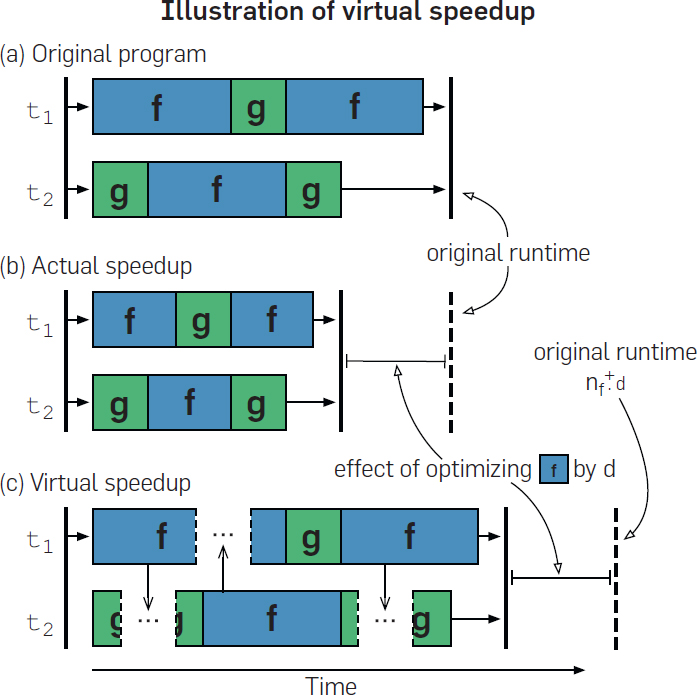
\includegraphics[width=0.6\textwidth]{images/virtual-speedup.jpg}
\end{center}

\end{frame}


\begin{frame}
\frametitle{Coz Graphs}

\begin{center}
	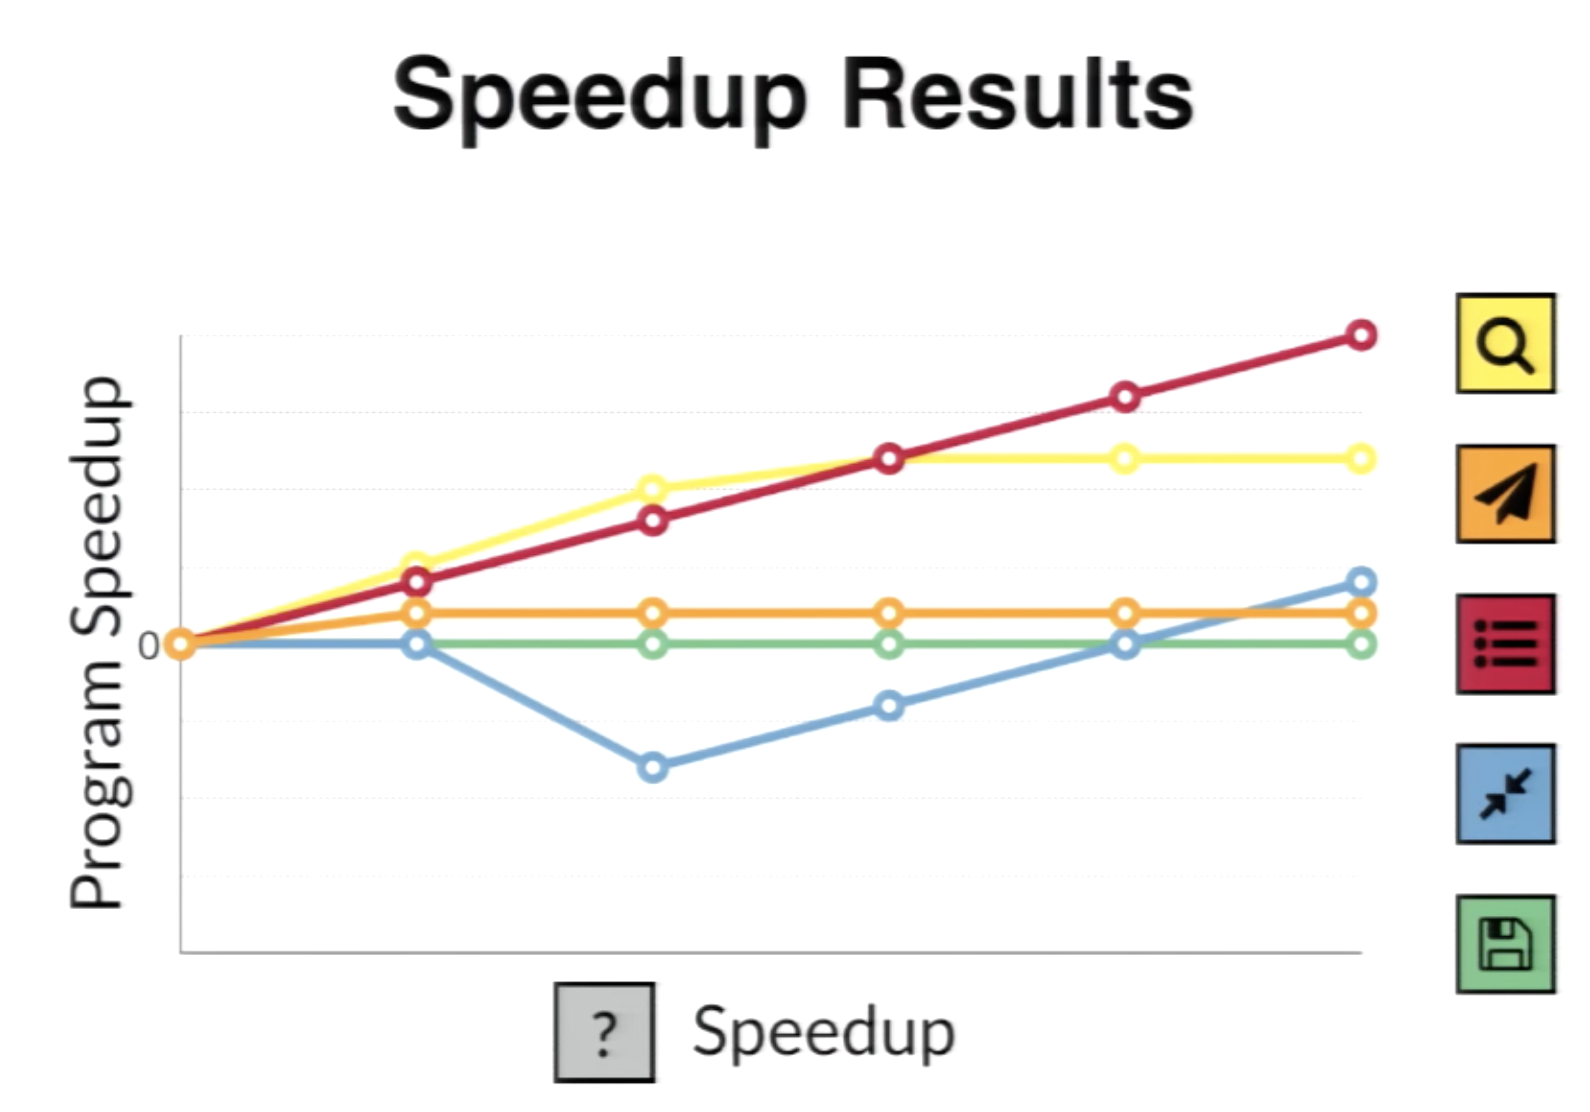
\includegraphics[width=\textwidth]{images/coz-speedup-graph.png}
\end{center}

\end{frame}


\begin{frame}
\frametitle{That Would Be Nice}
Just because hypothetically speeding up a particular part of the program would be beneficial, doesn't mean that it's possible to speed up that part.

We still need to assess what we can do and how difficult it would be.

\end{frame}


\begin{frame}
\frametitle{Does it Work?}

\begin{center}
	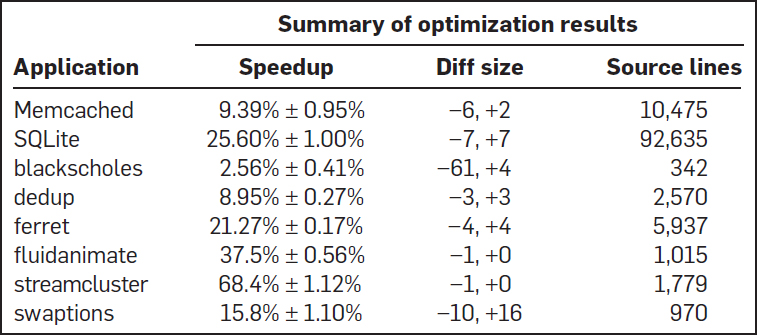
\includegraphics[width=\textwidth]{images/coz-speedup.jpg}
\end{center}

\end{frame}


\begin{frame}
\frametitle{Limitations, Overhead}

Only works on one machine where we have access to all threads.

Estimated overhead is 17.6\% total:\\
\quad 2.6\% startup debug information collection\\
\quad 4.8\% sampling\\
\quad 10.2\% inserted pauses

\end{frame}


\begin{frame}
\frametitle{More Details}

More details in the author presentation:

\url{https://www.youtube.com/watch?v=jE0V-p1odPg}

\end{frame}



\begin{frame}
\frametitle{\st{Memory Profiling} Return to Asgard}

\large

As with queueing theory:\\
\qquad allocs $>$ frees $\Longrightarrow$ usage $\rightarrow \infty$

At least more paging, maybe total out-of-memory.

But! Memory isn't really lost: we could free it.

Our tool for this comes from the Valgrind tool suite.


\end{frame}


\begin{frame}
\frametitle{DHAT}
DHAT tracks allocation points and what happens to them over a program's execution. 

An allocation point is a point in the program which allocates memory.

\end{frame}


\begin{frame}[fragile]
\frametitle{Leaf Node}

{\scriptsize
\begin{verbatim}
AP 1.1.1.1/2 {
  Total:     31,460,928 bytes (2.32%, 1,565.9/Minstr) in 262,171 blocks (4.41%, 13.05/Minstr), 
     avg size 120 bytes, avg lifetime 986,406,885.05 instrs (4.91% of program duration)
  Max:       16,779,136 bytes in 65,543 blocks, avg size 256 bytes
  At t-gmax: 0 bytes (0%) in 0 blocks (0%), avg size 0 bytes
  At t-end:  0 bytes (0%) in 0 blocks (0%), avg size 0 bytes
  Reads:     5,964,704 bytes (0.11%, 296.88/Minstr), 0.19/byte
  Writes:    10,487,200 bytes (0.51%, 521.98/Minstr), 0.33/byte
  Allocated at {
    ^1: 0x95CACC9: alloc (alloc.rs:72)
      [omitted]
    ^7: 0x95CACC9: parse_token_trees_until_close_delim (tokentrees.rs:27)
    ^8: 0x95CACC9: syntax::parse::lexer::tokentrees::<impl syntax::parse::lexer::
                          StringReader<'a>>::parse_token_tree (tokentrees.rs:81)
    ^9: 0x95CAC39: parse_token_trees_until_close_delim (tokentrees.rs:26)
    ^10: 0x95CAC39: syntax::parse::lexer::tokentrees::<impl syntax::parse::lexer::
                          StringReader<'a>>::parse_token_tree (tokentrees.rs:81)
    #11: 0x95CAC39: parse_token_trees_until_close_delim (tokentrees.rs:26)
    #12: 0x95CAC39: syntax::parse::lexer::tokentrees::<impl syntax::parse::lexer::
                          StringReader<'a>>::parse_token_tree (tokentrees.rs:81)
  }
}
\end{verbatim}
}


\end{frame}


\begin{frame}
\frametitle{Parents}
 Going up the tree, DHAT tells you about all of the allocation points that share a call-stack
prefix. 

The \texttt{\^} before the number indicates that the line is copied from the parent.

A \# indicates that the line is unique to that node.

A sibling of the example above would diverge at the call on line 10.

\end{frame}



\begin{frame}
\frametitle{Shieldmaiden to Thor}

\begin{center}
	\includegraphics[width=\textwidth]{images/Sif.jpg}
\end{center}

\end{frame}



\begin{frame}
\frametitle{Using Massif}

\Large

What does Massif do? 

\begin{itemize}
\item How much heap memory is your program using?
\item How did this happen?
\end{itemize}

Next up: example from Massif docs.



\end{frame}

\begin{frame}[fragile]
\frametitle{Example Allocation Program}


\begin{lstlisting}[language=Rust]
fn g() {
    let a = Vec::<u8>::with_capacity(4000);
    std::mem::forget(a)
}

fn f() {
    let a = Vec::<u8>::with_capacity(2000);
    std::mem::forget(a);
    g()
}

fn main() {

    let mut a = Vec::with_capacity(10);
    for _i in 0..10 {
	a.push(Box::new([0;1000]))
    }
    f();
    g();
}
\end{lstlisting}

\end{frame}

\begin{frame}[fragile]
\frametitle{Send in Sif}

After we compile, run the command:
{\scriptsize
\begin{verbatim}
plam@amqui ~/c/p/l/l/L/alloc> valgrind --tool=massif target/debug/alloc
==406569== Massif, a heap profiler
==406569== Copyright (C) 2003-2017, and GNU GPL'd, by Nicholas Nethercote
==406569== Using Valgrind-3.16.1 and LibVEX; rerun with -h for copyright info
==406569== Command: target/debug/alloc
==406569== 
==406569== 
\end{verbatim}
}
\end{frame}


\begin{frame}
\frametitle{That Was Useful!!!}

\large

What happened? 

\begin{enumerate}
\item The program ran slowly (because Valgrind!)

\item No summary data on the console \\
\hspace*{2em} (like memcheck or helgrind or cachegrind.)
\end{enumerate}

Weird. What we got instead was the file \texttt{massif.out.[PID]}.


\end{frame}


\begin{frame}
\frametitle{Post-Processing}

\Large

\texttt{massif.out.[PID]}:\\
\hspace*{2cm} plain text, sort of readable.

Better: \texttt{ms\_print}.

Which has nothing whatsoever to do with Microsoft. Promise.


\end{frame}


\begin{frame}[fragile]
\frametitle{Post-Processed Output}
{\scriptsize
\begin{verbatim}

    KB
19.71^                                                                       #
     |                                                                       #
     |                                                                       #
     |                                                                       #
     |                                                                       #
     |                                                                       #
     |                                                                       #
     |                                                                       #
     |                                                                       #
     |                                                                       #
     |                                                                       #
     |                                                                       #
     |                                                                       #
     |                                                                       #
     |                                                                       #
     |                                                                       #
     |                                                                      :#
     |                                                                      :#
     |                                                                      :#
     |                                                                      :#
   0 +----------------------------------------------------------------------->ki
     0                                                                   111.9
\end{verbatim}
}
\end{frame}


\begin{frame}[fragile]
\frametitle{User Friendly, But Not Useful}

\Large

For a long time, nothing happens, then\ldots kaboom! 

Why? We gave it a trivial program.

We should tell Massif to care more \\
about bytes than CPU cycles,\\
with \verb+--time-unit=B+.

Let's try that.



\end{frame}


\begin{frame}
\frametitle{Valgrind (Memcheck) First}


Run valgrind (Memcheck) first and make it happy \\
before we go into figuring out where heap blocks are going with Massif. 

Okay, what to do with the information from Massif, anyway? 

Easy!
\begin{itemize}
\item Start with peak (worst case scenario) \\ and see where that takes you (if anywhere). 

\item You can probably identify some cases where memory is hanging around unnecessarily. 
\end{itemize}



\end{frame}


\begin{frame}
\frametitle{Places to Look with Massif}

\large
Memory usage climbing over a long period of time, perhaps slowly, but never decreasing---memory filling with junk? 

Large spikes in the graph---why so much allocation and deallocation in a short period?
\end{frame}



\begin{frame}[fragile]
\frametitle{Other Massif-ly Useful Things}

\large
\begin{itemize}
	\item stack allocation (\verb+--stacks=yes+).
	\item children of a process \\ (anything split off with \texttt{fork}) if desired.
	\item low level stuff: if going beyond \texttt{malloc}, \texttt{calloc}, \texttt{new}, etc. and using \texttt{mmap} or \texttt{brk} that is usually missed, can do profiling at page level (\verb+--pages-as-heap=yes+).
\end{itemize}

\end{frame}




\begin{frame}
\frametitle{Live Demos}

\large

As is often the case, \\ we have examined the tool on a trivial program. 

Let's see if we can do some\\
 live demos of Massif at work.

\end{frame}


\end{document}


